We evaluate our three proposed algorithms( RS, LB, SP),
using extensive simulations on the real-world Abilene network
topology \cite{13} with 11 nodes and 14 links. We consider the
Abilene network to be a representative example of a small scale networks in practice.
The simulator is based on SimPy and is tested with Python 3.8. We set randomly pick heterogeneous node capacities
$capv \in (0, 7, 14)$ .

Furthermore, we consider the SFCs $(a,b,c)$ all with mean processing delay $processorDelayMean = 5$ and standard deviation $stdev=0$


Furthermore, they incur a per-flow processing delay that is
normally distributed with N (5 ms, 1 ms), where values are
cut off at 0 ms to prevent negative delays. Flows arriving
at the network's ingress nodes request one of the three
services chosen uniformly at random. For each ingress,
flow inter-arrival times mean is set to 12 , flow duration $df_mean=1$ , and flow data rate standard deviation is set to 0. The duration per experiment is 
$|T| = 100$ time steps.

The file structure of the simulator is as follows\cite{14}: - docs (Folder): Contains the documentation files of the project. - params (Folder): Contains sample parameter files
 (network file and VNF file) for testing purposes. - src (Folder): Contains the source
  code for the simulator and the interface. - coordsim (Folder): contains the source code
   of the simulator - metrics (Folder): contains the metrics module. - network (Folder):
   contains the network module. - reader (Folder): contains the params file reader module.
   - simulation (Folder): main simulator module. - main (Python): main executable for running the simulator from CLI - siminterface (Folder): contains the interface source code
    - tests (Folder): contains the unit tests for the simulator.

The simulator works as follows: The user (coordination algorithm or cli) provide two main inputs for the simulator: - Network file: GraphML file using the Zoo format. This file
contains the network nodes and the edges. - VNF file: YAML file that includes the list of
SFCs and the list of SFs under each SFC in an ordered manner. The file can also include
a specified placement that can be used as a default placement. The SFs must include a
processing delay mean and standard deviation values so that processing delays can be
calculated for each flow passing through that SF.

Once the parameters are provided, the flow of data through the simulator is as follows:
\begin{itemize}
\item The input network and VNF files are parsed producing a NetworkX object containing the list of nodes and edges, and the shortest paths of the network (using Floyd-Warshall). The
parsing also produces dictionaries that contain the list of SFCs and the list of SFs and
their respective values. Additionally, the list of ingress nodes (nodes at which flows
arrive) are also calculated from the GraphML file. These parameters are then passed to a
SimulatorParams object, which holds all the parameters of the simulator, the simulator is then started using the FlowSimulator object's start() $function$.

\item At each ingress node, the $function$ $generate_flow$ is called as a SimPy process, this
$function$ creates Flow objects with exponentially distributed random inter arrival times.
The flow's data rate and size are generated using normally distributed random variables.
All of the inter arrival time, data rate, and flow size parameters are user configurable.
The flow is also assigned a random SFC chosen from the list of available SFC given in the VNF file.

\item Once the flow is generated, $init_flow()$ is called as a SimPy process which initializes
the handling of the flow within the simulator. The $function$ then calls $pass_flow()$, which
then handles the scheduling of the flow according to the defined load balancing rules
(flow schedule). Once the next node has been determined, the forwarding of the flow is
simulated by halting the flow for the path delay duration using the $forward_flow()$
$function$. Once that is done, the processing of the flow is simulated by calling
$process_flow()$ as a SimPy process. If the requested SF was not found at the next
 node, the flow is then dropped.

\item In $process_flow()$, the processing delay for that particular SF is generated using
given
mean and standard deviation values using a normal distribution. The simulator checks the
node?s remaining processing capacity to check if the node can handle the data rate
requested by the SF, if there is not enough capacity, then the flow is dropped. For the
duration that the flow is being processed by the SF, the flow's data rate is deducted from the node's capacity, and returned after the flow finished processing completely.

\item Once the flow was processed completely at each SF, $depart_flow()$ is called to
register the flow's departure from the network. If the flow still has other SFs to be
processed at
in the network, $process_flow()$ calls $pass_flow()$ again in a mutually recursive manner.
This allows the flow to stay in the SF for processing, while the parts of the flow that
were processed already to be sent to the next SF.
\end{itemize}

\textbf{Input Parameters:} 
The available input parameters that are configurable by the user are: - d: The duration of the simulation (simulates milliseconds). - s: The seed to use for the random number
generator. - n: The GraphML network file that specifies the nodes and edges of the
 network. - sf: VNF file which contains the SFCs and their respective SFs and their properties. - iam: Inter arrival mean of the flows' arrival at ingress nodes. - fdm: The
 mean value for the generation of data rate values for each flow. - fds: The standard
deviation value for the generation of data rate values for each flow. - fss: The shape of the Pareto distribution for the generation of the flow size values.

\begin{figure}[h]
    \centering
    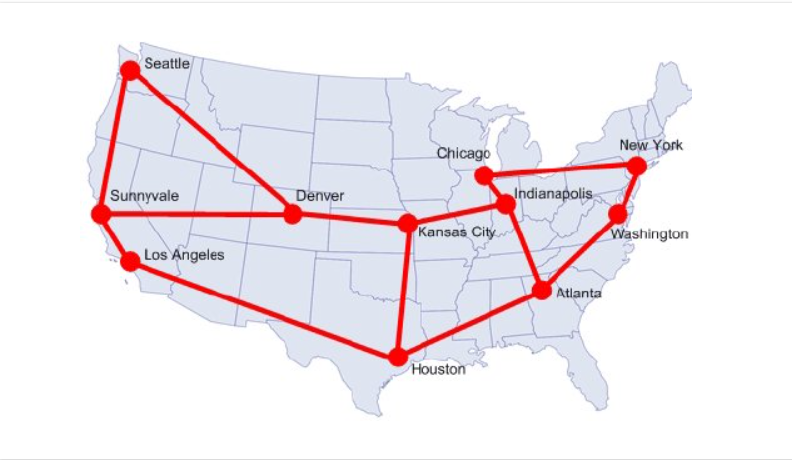
\includegraphics[width=1\textwidth]{abilene_real}
    \caption{Abilene topology graph}
    \label{fig:abilene_real}
\end{figure}


